\chapter{Исследование управляемости}
\label{ch:chap1}
\section{Условие задачи}

Необходимо рассмотреть систему:
$$
  \dot{x} = Ax + Bu
$$ и выполнить следующие шаги:

\begin{itemize}
\item  Исследовать управляемость системы:
  \begin{itemize}
    \item Найти матрицу управляемости системы, определить ее ранг, сделать вывод об управляемости системы в целом.
    \item Найти собственные числа матрицы A, найти для каждого из собственных чи
    сел матрицу Хаутуса (для управляемости), определить ранги матриц, сделать
     выводы об управляемости каждого собственного числа и системы в целом.
     \item Найти Жорданову (или диагональную) форму системы и сделать выводы об
     управляемости каждого собственного числа и системы в целом.
  \end{itemize}
  \item Найти Грамиан управляемости системы относительно времени $t_1 = 3$, вычислить
  его собственные числа. Проанализировать полученные собственные числа с точки
  зрения управляемости системы.
  \item Найти управление, переводящее систему из $x(0) = 0$ в $x(t_1) = x_1$ за время $t_1$. Вы
  полнить моделирование системы, демонстрирующее корректность выполненных
   расчетов
\end{itemize}

\section{Решение задачи}

Параметры для объекта:
$$
  A = \begin{bmatrix}
  3 & -6 & 4 \\
  4 & -5 & 4 \\
  -4 & 4 & -5 
  \end{bmatrix} \tab
  B = \begin{bmatrix}
    -1 \\ 3 \\ 1 
  \end{bmatrix} \tab
  x_1 = \begin{bmatrix}
  1 \\ 0 \\ 0
  \end{bmatrix} 
$$

\subsection{Исследование управляемости системы}

Найдем матрицу управляемости системы:

$$
    U = \begin{bmatrix}
      B & AB & A^2B
    \end{bmatrix} =  \begin{bmatrix}
      -1 & -17 & 83 \\
      3 & -15 & 51 \\
      1 & 11 & -47
    \end{bmatrix}
$$
$$
  rank(U) = 3
$$
В таком случае по критерию Калмана, наша система полностью управляема по состоянию, так как ранк матрицы управляемости равен порядку системы.

Найдём собственные числа матрицы $A$:
$$
    \lambda_{1,2} = -3 \pm 2i, \tab \lambda_3 = -1 
$$

Вычислим матрицу Хаутуса для каждого собственного числа:
$$
    H_1 = \begin{bmatrix}
          A - \lambda_1 I & B   
          \end{bmatrix} = 
    \begin{bmatrix}
    6-2i & -6 & 4 & -1 \\  
    4 & -2-2i & 4 & 3 \\  
    -4 & 4 & -2 -2i & 1   
    \end{bmatrix}
$$
$$
rank(H_1) = 3
$$
Значит собственное число $\lambda_1$ является управляемым, если ранг его матрицы Хаутуса равняется порядку системы.
$$
    H_2 = \begin{bmatrix}
          A - \lambda_2 I & B   
          \end{bmatrix} = 
    \begin{bmatrix}
      6+2i & -6 & 4 & -1 \\  
      4 & -2+2i & 4 & 3 \\  
      -4 & 4 & -2+2i & 1  
    \end{bmatrix}
$$
$$
rank(H_2) = 3
$$
Аналогично, собственное число $\lambda_2$ является управляемым.
$$
    H_3 = \begin{bmatrix}
          A - \lambda_3 I & B   
          \end{bmatrix} = 
    \begin{bmatrix}
      4 & -6 & 4 & -1 \\
      4 & -4 & 4 & 3 \\
      -4 & 4 & -4 & 1
    \end{bmatrix}
$$
$$
rank(H_3) = 3
$$
Аналогично, собственное число $\lambda_3$ является управляемым. В итоге, так как все собственные числа матрицы $A$ - управляемые, значит и система полностью управляема.

Теперь найдём Жорданову форму системы, в общем виде она выглядит следующим образом:
$$
    \begin{cases}
      \dot{\hat{x}} = P^{-1}\boldsymbol{A}P \hat{x} + P^{-1}\boldsymbol{B} u \\
      y = CP\hat{x}
    \end{cases}
$$
Система в жордановой форме полностью управляема тогда и только тогда, когда
\begin{itemize}
  \item Все жордановы клетки относятся к различным собственным числам
  \item Элементы матрицы входных воздействий, соответствующие \dots
  \begin{itemize}
    \item $\mathbb{R}$ случай: последним строкам жордановых клеток, не равны нулю.
    \item $\mathbb{C}$ и не кратные, случай: верхняя или нижняя строка жордановых клеток, не равны нулю.
    \item $\mathbb{C}$ и кратные, случай: обе нижние строки жордановых клеток, не равны нулю.
  \end{itemize}
\end{itemize}

В нашем случае жорданова клетка и входное воздействие таково:
$$
    \mathbf{A} = \begin{bmatrix}
        -1 & 0 & 0 \\
        0 & -3 & -2 \\
        0 & 2 & -3 
        \end{bmatrix} \tab 
    P^{-1}B = B^* = \begin{bmatrix}
        4 \\ -1.5+1.5i \\ -1.5-1.5i
        \end{bmatrix}
$$

Как можно заметить, оба собственных числа соответствуют различным жордановым клеткам, и для каждой из них строка матрицы входных воздействий не равна нулю.
Значит эти три собственных числа управляемы, и как следствие - вся система полностью управляема. 

\subsection{Грамиан управляемости}

Грамиан управляемости системы относительно времени $t_1 = 3$:

$$
P(t_1) = \int_{0}^{t_1}e^{At}BB^Te^{A^Tt}dt = 
    \begin{bmatrix}
      8.78 & -0.5 & -7.47 \\ 
      -0.5 & 0.8 & 0.39 \\ 
      -7.47 & 0.39 & 6.38  
    \end{bmatrix}
$$

Его собственные числа:
$$
    p_{1} = 0.01 , \tab p_{2} = 0.78, \tab p_3 = 15.18
$$
Как можно заметить, они все положительные, а это значит, что она положительно определена. 
Также это значит, что её определитель положительный.

Грамиан управляемости должен быть невырожден во все моменты времени:
$$
\forall t_1 > 0, \rightarrow det\bigg( \int_{0}^{t_1}e^{A^Tt}C^TCe^{At}dt \bigg) > 0
$$
В нашем случае это тоже выполняется, тогда система полностью управляема.

\subsection{Моделирование управления}

Рассчитаем управление, переводящее систему из $x(0) = 0$ в $x(t_1) = x_1$ за время $t_1$:
$$
    u(t) = B^T e^{A^T(t_1 - t)}(P(t_1))^{-1}x_1 = 
$$
\begin{figure}[ht]
    \centering
    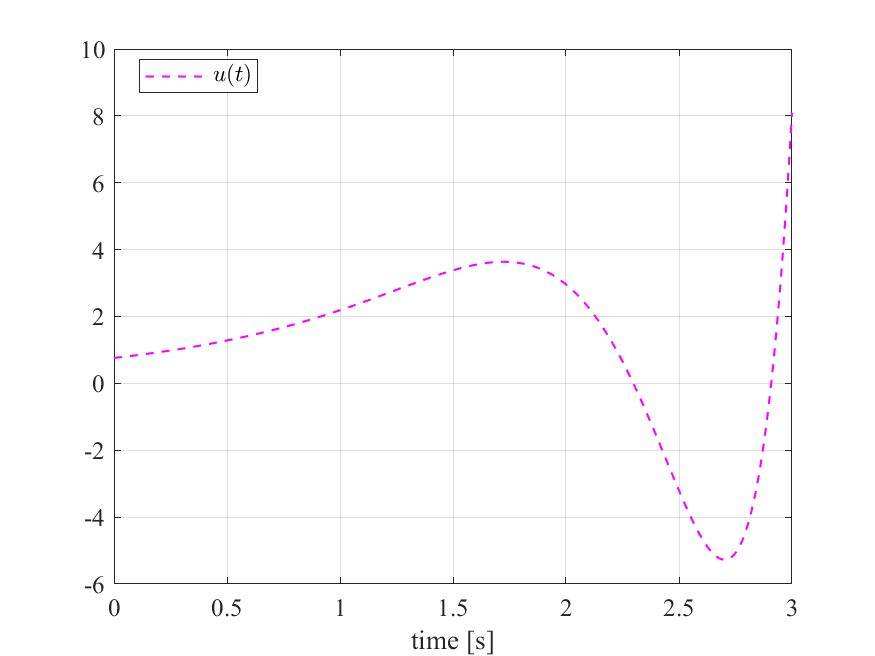
\includegraphics[width=1.0\textwidth]{control1.png}
    \caption{Управляющий сигнал}
\end{figure}

Вектор состояний системы будет выглядеть следующим образом:
\begin{figure}[ht]
  \centering
  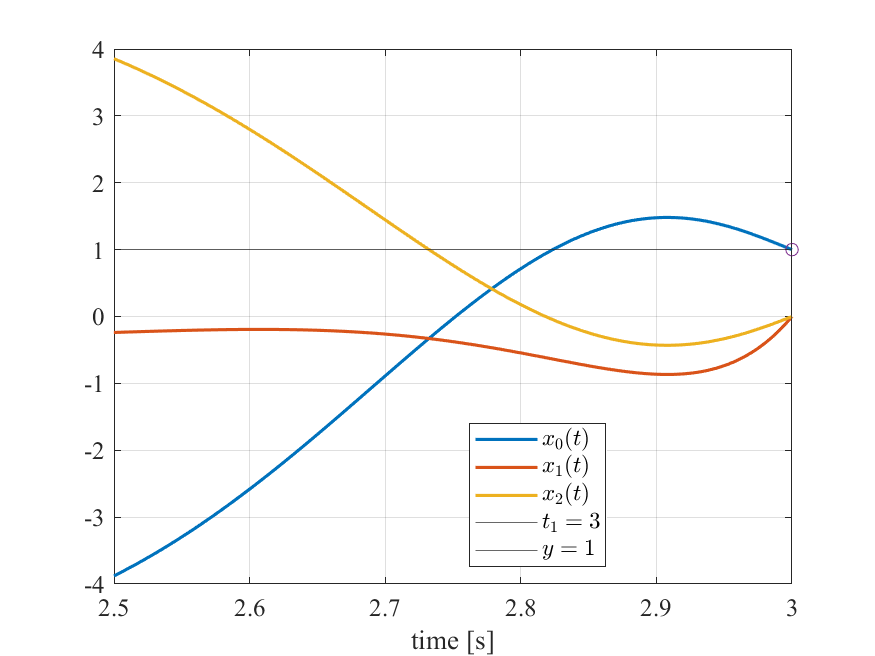
\includegraphics[width=1.0\textwidth]{controlability1.png}
  \caption{Состояния системы}
\end{figure}

Видно, что система управляемая в соответствии с заданным управлением и переходит в заданное состояние в нужный момент времени.

\subsection{Вывод}

Исследование системы задания показало, что она является полностью управляемой. 
Это было продемонстрировано с помощью критерия Калмана, через управляемость всех собственных значений и жорданову форму системы.
Ещё был найден грамиан управляемости и проверены его собственные числа. 
Проведено моделирование системы с управлением, которое переводит систему в заданное состояние. Результаты такого моделирования показали,
что что система управляема и программное управление работает корректно.
\endinput